\documentclass[aspectratio=169, pdf, 8pt, unicode]{beamer}
\usepackage[american,russian]{babel}
\usepackage[default]{sourcesanspro}
\usepackage{float}
\usepackage{graphicx}
\usepackage{pgfplotstable}
\usepackage{caption}
\usepackage{amsmath}
\usepackage{amssymb}
\usepackage{setspace}
\usepackage{fancyvrb}
\usepackage[outputdir=aux]{minted}
\usepackage{url}

\DeclareCaptionLabelFormat{gostfigure}{Рисунок #2}
\captionsetup[table]{labelsep=endash,justification=justified,singlelinecheck=false,font=normalsize,skip=0pt} 
\captionsetup[figure]{labelformat=gostfigure,labelsep=endash,justification=centering,singlelinecheck=false,font=normalsize} 
\pgfplotsset{compat=1.9}

\mode<presentation> {
\usetheme{Madrid}
}

\setbeamerfont{institute}{size=\normalsize}
\setbeamertemplate{itemize/enumerate body begin}{\large}
\setbeamertemplate{itemize/enumerate subbody begin}{\tiny}

\title[Теория и практика многопоточного программирования]{Теория и практика многопоточного программирования}

\author{Неганов Алексей}

\institute[МФТИ]{
    Московский физико-технический институт (национальный исследовательский университет)\\
    Кафедра теоретической и прикладной информатики\\
}

\date{Москва 2020}

\setbeamertemplate{caption}[numbered]

\begin{document}

\begin{frame}
\titlepage
\end{frame}

\begin{frame}[fragile]
\frametitle{Lock-free ordered list}
\begin{figure}[H]
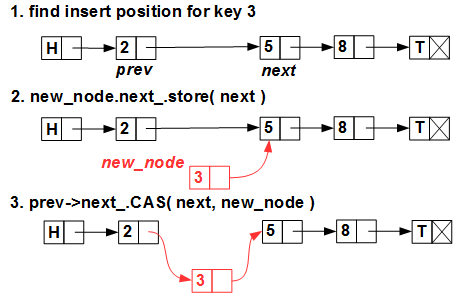
\includegraphics[width=0.5\textwidth]{fig/lfol1.png}
\end{figure}
\end{frame}

\begin{frame}[fragile]
\frametitle{Lock-free ordered list}
\begin{figure}[H]
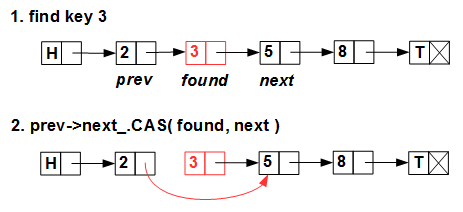
\includegraphics[width=0.5\textwidth]{fig/lfol2.png}
\end{figure}
\end{frame}

\begin{frame}[fragile]
\frametitle{Lock-free ordered list}
\begin{figure}[H]
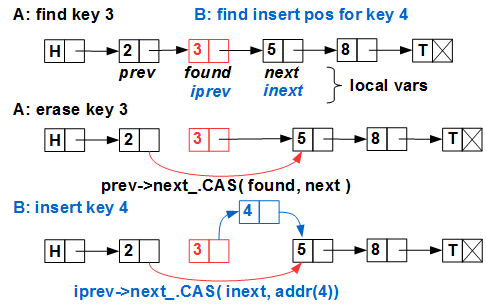
\includegraphics[width=0.5\textwidth]{fig/lfol3.png}
\end{figure}
\end{frame}

\begin{frame}[fragile]
\frametitle{Lock-free ordered list}
\begin{figure}[H]
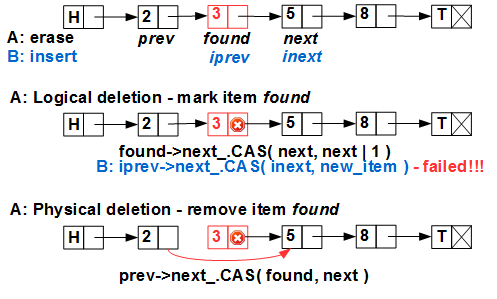
\includegraphics[width=0.5\textwidth]{fig/lfol4.png}
\end{figure}
\end{frame}

\begin{frame}[fragile]
\frametitle{Hash tables}
\begin{figure}[H]
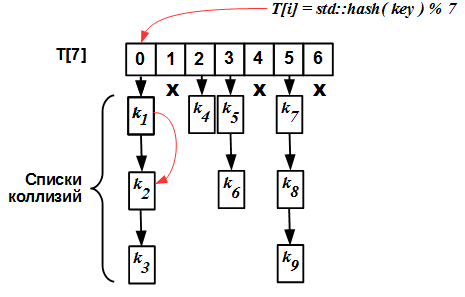
\includegraphics[width=0.5\textwidth]{fig/hashtable.png}
\end{figure}
\end{frame}

\begin{frame}[fragile]
\frametitle{Striping}
\begin{figure}[H]
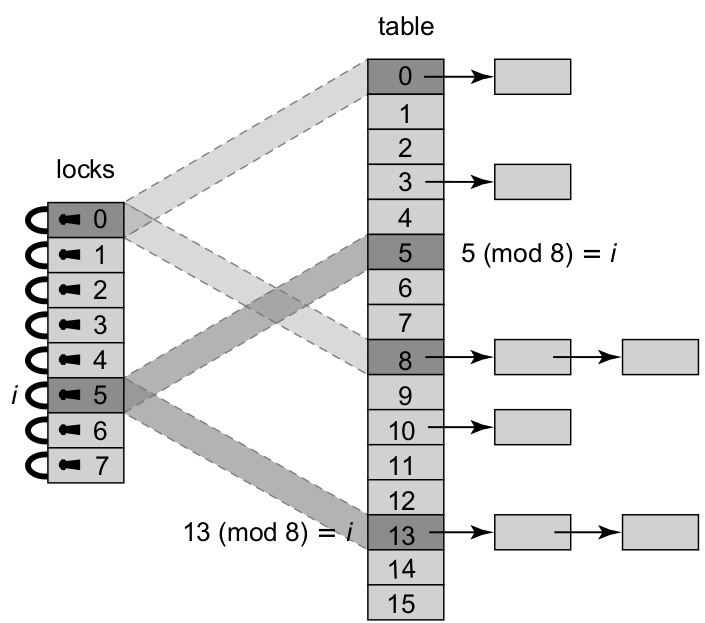
\includegraphics[width=0.5\textwidth]{fig/striping.png}
\end{figure}
\end{frame}

\begin{frame}[fragile]
\frametitle{Split-ordered list}
\begin{figure}[H]
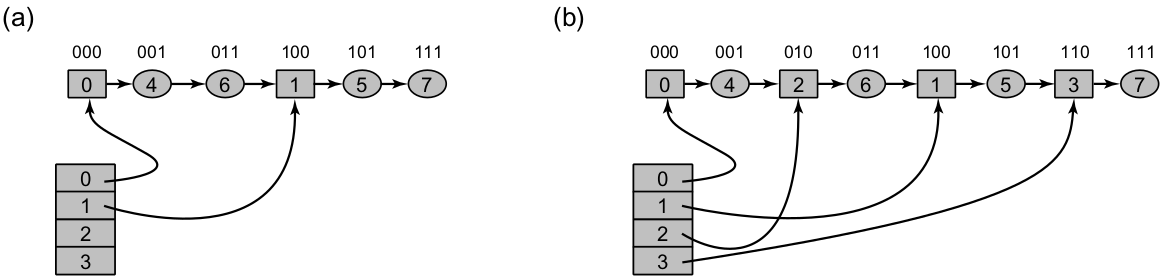
\includegraphics[width=0.8\textwidth]{fig/split-ordered.png}
\end{figure}
\end{frame}

\begin{frame}[fragile]
\frametitle{Split-ordered list}
\begin{figure}[H]
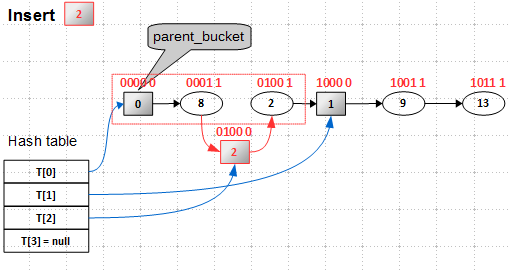
\includegraphics[width=0.5\textwidth]{fig/split-ordered-1.png}
\end{figure}
\end{frame}

\begin{frame}[fragile]
\frametitle{Split-ordered list}
\begin{figure}[H]
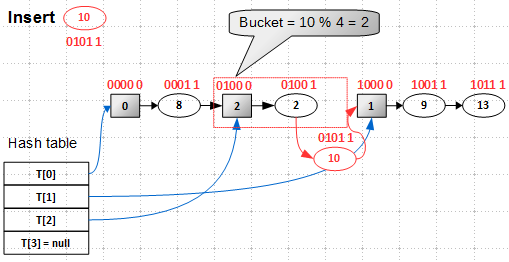
\includegraphics[width=0.5\textwidth]{fig/split-ordered-2.png}
\end{figure}
\end{frame}

\end{document}
